\documentclass[a4paper, ngerman, 12pt]{scrartcl}
\usepackage[backend=biber, style=verbose-trad2]{biblatex}
% shell-escape
% TODO: [ ] Was ist eine REST-API
%	[ ] Hosten definiren
%	[x] Database erklären (sql vs. noSql)
%	[ ] JSON Erklären
%	[ ] Mikrokontroler
% Setup {{{1
% Packages {{{2
%\usepackage[top=4cm, left=3.5cm, right=2.5cm, bottom=4.5cm]{geometry}
\usepackage{amsfonts, amsmath, amssymb}
\usepackage{minted}
\usepackage{babel}
\usepackage{graphicx}
\usepackage{float}
\usepackage[utf8]{inputenc}
\usepackage{fancyhdr}
\usepackage{tikz}
\usepackage[RPvoltages]{circuitikz}
\usepackage{csquotes}
\usepackage{xpatch}
\usepackage[gen]{eurosym}
%\usepackage{mathptmx}
%\usepackage[scaled=0.9]{helvet}
%\usepackage{courier}
\usepackage[T1]{fontenc}
\usepackage{lmodern}
\usepackage[breaklinks=true]{hyperref}
\usepackage{wrapfig}
\usepackage[onehalfspacing]{setspace}
% Minted {{{2
\definecolor{bg}{rgb}{0.95,0.95,0.95}
%\usemintedstyle{solarized-dark}
% Heading {{{2
\pagestyle{fancy}
\fancyhead{}
\fancyfoot{}
\fancyhead[L]{\slshape \MakeUppercase{Informatik Jahresarbeit}\/}
\fancyhead[R]{\slshape Jasper Levin Spahl\/}
\fancyhead[C]{\thepage}
% Paragraph {{{2
%\parindent 0ex
\setlength{\parindent}{1em}
\setlength{\parskip}{1em}
\renewcommand{\baselinestretch}{1.1}
% }}}
% Makro {{{2
\newcommand{\js}[1]{\mintinline{javascript}{#1}}
% }}}
\author{Jasper Levin Spahl}
% Tikz Setup {{{2
\usetikzlibrary{shapes.geometric, arrows.meta}
% Bibliograthy Setup {{{2
\addbibresource{quellen.bib}
\begin{document}
% Titlepage {{{2
\begin{titlepage}
\begin{center}
\vspace*{1cm}

\Large{\textbf{Informatik}}\\
\Large{\textbf{Jahresarbeit}}\\
\vfill
\line(1,0){400}\\[1mm]
\huge{\textbf{Der Smarte Bienenstock}}\\[3mm]
\large{Entwicklung eines Serversystems für eine Bienenstockwaage}\\[3mm]
\Large{\textbf{- 12 Kss -}}\\
\line(1,0){400}\\
\vfill
Jasper Levin Spahl\\
Klasse: 12Kss\\
\today\\
\end{center}
\end{titlepage}

% Table of contents {{{2
\tableofcontents
\thispagestyle{empty}
\clearpage
\setcounter{page}{1}

% Einleitung {{{1
\section{Einleitung}

Bei der Auswahl des Themas meiner Jahresarbeit war ich lang unentschlossen.
Ich wusste sofort, dass ich entweder etwas kreatives oder etwas im It-Bereich machen wollte.
Meine erste Idee war es einen Lichtwecker zubauen.
Ich bemerkte jedoch als ich damit fast fertig war das, dass ganze sehr viel leichter umzusetzen war, sodass ich damit keine komplette Jahresarbeit füllen konnte.
Mir gefiel allerdings das Thema Smarthome/Homeautomation.
Letztendlich brachte mich mein Vater auf die Idee.
Er erzählte mir vom einem Freunde der eine Bienenstockwaage besitzt.
Mit hilft so einer Bienenstockwaage kann man überwachen wie viel Honig sich gerade in dem Stock der auf ihr steht befindet.
Diese Waagen kosten zwischen 800 und 3000 \euro{}, sind somit viel zu überteuert.

Wenn man jedoch eine billigere Version haben will muss man sie sich selbst bauen.
Es gibt zwar, wie ich später herausfand, eine relative einfache Bauanleitung für ein solches System.
~\autocite{Honeypi}
Allerdings benötigt dieses System einen Anschluss an eine Cloud, dessen Source Code nicht offen ist.
Das heißt die Daten werden an irgendeinen Server übermittelt der sie dann speichert.
Man weiß also nicht er alles auf die Daten zugreifen kann.
Diese potenzielle Sicherheitslücke hat man nicht, wenn man das ganze selbst entwickelt.

% Wichtige Begriffe {{{1
\section{Wichtige Begriffe}
Da ich in meiner Jahresarbeit über komplexere Konzepte benutze ist diese kurze Begriffserklärung notwendig.

% Was ist ein Server? {{{2
\subsection{Was ist ein Server?}
Der Begriff \enquote{\textbf{Server}} (englisch für \textit{Diener}) hat zwei Bedeutungen.
Es gibt Hardware und Soft\-ware-Ser\-ver.
Als \textbf{Soft\-ware-Ser\-ver} bezeichnet man ein Programm, das einen speziellen Dienst anderen Programmen, sogenannten Clients (englisch für \textit{Kunden}), zur Verfügung stellt.
Ein Webserver zum Beispiel, stellt eine Internetseite ins Netz.~\autocite[ver.][]{IonosServer}

Wenn die meisten Leute an einen Server denken, haben sie eine große Serverfarm im Kopf.
Doch ein Hard\-ware-Ser\-ver muss nicht unbedingt groß sein und viel Strom verbrauchen.
Ein \textbf{Hard\-ware-Ser\-ver}, auch \textit{Host} genannt, definiert sich dadurch dass auf ihm einer oder mehrere Soft\-ware-Ser\-ver laufen. Das heißt jeder Computer, jedes Smartphone kann ein Server sein.
Selbst einen modernen Kühlschrank kann man heute zu Tage als Server bezeichnen solange er eine Serversoftware benutzt um z.B. zu zeigen, was man alles bei deinem nächsten Einkauf mitbringen musst.

% Was ist eine API {{{2
\subsection{Was ist eine API?}\label{sec:api}

Eine \textbf{API}, kurz für \enquote{\textbf{Application Programming Interface}}\footnote{englisch für \textit{An\-wen\-dungs\-pro\-gram\-mier Schnittstelle}}, ist eine Schnittstelle die es Programmen, und Hardware ermöglicht mit einander zu kommunizieren.
Eine API kann von Anwendungsbereich zu Anwendungsbereich komplett verschieden sein.~\autocite[][]{GSApi}

% Es gibt viele veschidene Standarts eine API zu programmieren.

In meiner Jahresarbeit habe ich vor allem \textbf{Web-APIs} benutzt.

% Was ist eine Programmiersprache {{{2
\subsection{Was ist eine Programmiersprache?}

Mit Hilfe von Programmiersprachen kann man einem PC sagen was er tun soll.
Die ersten Programmiersprachen wurden entwickelt um nicht alle Programme in Assembler\footnote{Die Befehle welche die CPU versteht} zu programmieren.
Es gibt viele verschiedene Programmiersprache die sich vor allem in vier Eigenschaften unterscheiden:

\begin{description}
	\item[Syntax] Wie werden Variablen definiert? Benutzt die Sprache viele Klammern oder Indentierung? Siehe Abbindung~\ref{abb:syntax}
	\item[Statische und Dynamische Typisierung] Muss man angeben welchen Type eine Variable hat?
	\item[Kompiliert vs Interpretiert] Wird der Quelltext zu einem binären Programm umgewandelt oder wird er mit einem sogenannten \textit{JIT-Compiler}\footnote{Just-in-time-Compiler} ausgeführt?
	\item[Höhe einer Programmiersprache] Die höhe einer Programmiersprache sagt aus wie nah sie an der Maschienensprache ist. Die Programmiersprache \emph{Python} zum Beispiel ist eine höhere Programmiersprache das bedeutet sie ist relative einfach zu programmieren. Sie wird eher für Automatisierungen benutzt. \emph{C} oder \emph{C++} hingengen sind sogenannte \emph{low level} Programmiersprachen. Diese Sprachen sind meist sehr schnell und werden vorallem zur Betriebssystemen und anderen hardwarenahen Anwendungen benutzt.
\end{description}

% abb:syntax {{{3
\begin{figure}[ht]
\begin{minipage}{0.5\textwidth}
\textbf{Python}
\begin{minted}[tabsize=4]{python}
def add(x, y):
	return x+y
print(add(1+2))
\end{minted}

\end{minipage}
\begin{minipage}{0.5\textwidth}
\textbf{Rust}
\begin{minted}[tabsize=4]{rust}
fn add(&x: i32, &y: i32) -> i32 {
	x+y
}
println!("{}", add(1,2));
\end{minted}
\end{minipage}
\begin{minipage}{0.5\textwidth}

\textbf{C++}

\begin{minted}[tabsize=4]{cpp}
int add(int x, int y) {
	return x + y;
}
int sum = add(1, 2);
std::cout << sum;
\end{minted}
\end{minipage}
\begin{minipage}{0.5\textwidth}
\textbf{Javascript}
\begin{minted}[tabsize=4]{javascript}
function add(x, y) {
	return x + y;
}
console.log(add(1,2));
\end{minted}
\end{minipage}

\caption{Syntax-Unterschiede in verschiedenen Programmiersprachen\label{abb:syntax}}
\end{figure}
% }}}

% Was ist Javascript {{{2
\subsection{Was ist Javascript?}

Javascript\footnote{abgekürzt als JS} ist eine Programmiersprache die dafür entwickelt wurde um Webseiten interaktiv zu gestalten.
Sie ist sehr einfach zu lernen, ist allerdings im Vergleich zu anderen Programmiersprachen ziemlich langsam.
Javascript ist eine dynamische Programmiersprache das heißt man muss den Variablen keinen bestimmten Type zuordnen.
Das ist zum schnellen programmieren zwar sehr gut, wird aber bei größeren Projekten zum Problem da man Fehler nicht so schnell findet.

% Datenbank {{{2
\subsection[Wo ist Datenbank? (Sql vs NoSql)]{Was ist eine Datenbank? Welche unterschiede gibt es?}

Eine Datenbank\footnote{abgekürzt als DB} ist ein Verwaltungssystem das große Mengen an Daten langfristig abspeichern und schnell wieder aufrufen kann.
Es gibt zwei unterschieliche Arten von Datenbanken. Die sogennaten \emph{SQL}- und \emph{NoSQL}-DBs.

\begin{description}
	\item[SQL-Datenbank] SQL steht für \enquote{\emph{Structured Query Language}}\footnote{dt: Struckturiere Abfrage Sprache}.
		SQL ist eine Sprache zum durchsuchen und endern des Inhaltes einer Datenbank.
		DBs die diese Sprache zur Verwaltung der Daten benutzen, speichern ihre Daten meist in speziellen Schemata z.B. Tabellen.
		Diese Tabellen haben meist verknüpfungen untereinander weswegen sie auch \enquote{relational} DBs genannt werde.
		Häufig genutzte Datenbanken sind MySQL, MariaDB und Postgres.
	\item[NoSQL-Datenbanken] Wie im Namen implementiert, benuzten diese DBs nicht SQL, sondern sie speichern ihre Daten in Dokumenten ab. Siehe Listing~\ref{lst:document}.
		Durch die nutzung von Dokumenten statt Schemata sind die Datenbanken flexibler.
		Sie benötigen dadurch allerdings eine komplexere Logik in der Anwendung.
\end{description}

\begin{listing}[H]
\begin{minted}[tabsize=2]{json}
{
	"_id": ObjectID,
	"name": "<name>",
	"data": [
		...,
		{
			"_id": ObjectID,
			"weight": 3505,
			"time": "2020-03-30T20:33:00.990+00:00"
		},
		...,
	]
}
\end{minted}
\caption{Dokument in Datenbank\label{lst:document}}
\end{listing}
% Funktionsweise meiner Bienenstockwaage {{{1
\section{Funktionsweise meiner Bienenstockwaage}
% Basic Funktionsweise {{{2

Eine Bienenstockwaage ist eigentlich recht einfach.
Im Grunde ist es nur eine Waage welche ihre Werte in regelmäßigen Abständen speichert bzw.
mit Hilfe von SMS oder Internet an den Betreiber übermittelt.

Im Falle meiner Bienenstockwaage habe ich mir ein System überlegt, das gut skalierbar ist.
Dieses System besteht aus mehreren Bestandteilen welche über verschiedene APIs mit einander kommunizieren.

Das wichtigste Element davon ist der Hauptserver auf dem die Datenbank MongoDB und der Webserver laufen.
Ich habe mir dafür einen Raspberry Pi 3B+ angeschafft, da ich alle Daten lokal speichern wollte.
Das muss man aber nicht, da man sich auch über die Plattform \href{https://www.mongodb.com/cloud/atlas}{MongoDB Atlas} eine Datenbank mieten kann und mit Hilfe von \href{https://www.linode.com}{Linode} oder \href{https://www.digitalocean.com/}{Digital Ocean} den Webserver hosten kann.

\begin{figure}[ht]
	\centering
	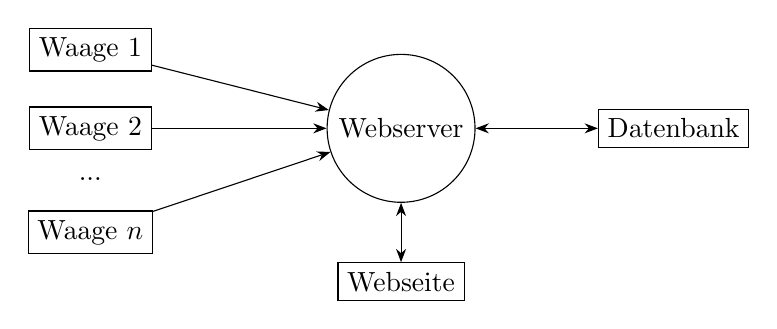
\begin{tikzpicture}

		\node[draw] (waage1) at (0,0) {Waage 1};
		\node[draw] (waage2) [below of = waage1] {Waage 2};
		\node[draw=none] (waage3) [below of = waage2, below = -0.5cm] {...};
		\node[draw] (waagen) [below of = waage3, below = -0.6cm] {Waage $n$};
		\node[draw, shape=circle] (server) [right of = waage2, right = 2cm] {Webserver};
		\node[draw] (app)    [below of = server, below = 0.7cm] {Webseite};
		\node[draw] (data)   [right of = server, right = 1.5cm] {Datenbank};

		\draw[-Stealth] (waage1) -- (server);
		\draw[-Stealth] (waage2) -- (server);
		\draw[-Stealth] (waagen) -- (server);
		\draw[Stealth-Stealth] (server) -- (data);
		\draw[Stealth-Stealth] (app) -- (server);
	\end{tikzpicture}
	\caption{Netzwerk Diagramm meines Serversystems\label{abb:networkdiagram}}
\end{figure}

Der Hauptbestanntteil meines Systems ist ein Zentraler Webserver welcher zur komonication mit der Webseite und den Bienenstockwaagen eine REST-API zur verfügung stellt.

% Die Waage {{{2
\subsection{Die Waage}

Die Bienenstockwaage funktioniert wie eine gewöhnliche Waage, welche man in dem meisten Haushalten findet.
Um zu verstehen, wie eine gewöhnliche Waage funktioniert muss man verstehen, wie eine Wägezelle funktioniert.

\begin{quote}
	\enquote{Wägezellen sind eine Sonderform der Kraftaufnehmer (Kraftsensoren) zum Aufbau von Wägevorrichtungen, d.h.\ zum Verwiegen mit Waagen.}~\autocite[vgl.][]{WikiWaegezelle}
\end{quote}

\begin{wrapfigure}{l}{7cm}
	\centering
	\begin{circuitikz}[european]
		\draw (0, 4) to[battery1] (0,0) -- (3,0) to[R] (1,2) to[R] (3,4) to[R] (5,2) to[R] (3,0);
		\draw (0,4) -- (3,4);
		\draw (1,2) to[short, -*] (2,2) node[right]{$V_0$};
		\draw (5,2) to[short, -*] (4,2) node[left]{$V_1$};
	\end{circuitikz}
	\caption{Schaltung der Wägezellen\label{abb:circuit}}

\end{wrapfigure}

Sie besteht aus einem Federkörper\footnote{Metallstück welches etwas flexibel ist}, auf dem ein Dehnungsmessstreifen\footnote{Im folgenden als DMS abgekürzt} fixiert ist.
Dieser DMS verändert je nach Dehnung seinen elektrischen Widerstand.
Wegen dieser Eingenschaft bekommt man,
wenn man mehrere Wägezellen wie in Abbildung~\ref{abb:circuit} gezeigt verkabelt und den Spannungsunterschied zwischen $V_0$ und $V_1$ misst,
einen Spannungsunsterschied der in Relation zu dem Gewicht auf den Wägezellen ist.

Der Spannungsunterschied wird nun von einem Digital- zu A\-na\-log-Um\-wandler in ein digitales Signal umgewandelt welches mit Hilfe eines Mikrokontrolers weiter verarbeitet werden kann.
Bei einer gewöhnlichen Waage wird der Wert meist mit einer Konstante multipliziert damit der Wert einer Masseinheit($kg$) entspricht. Dieser wird auf einem Bildschirm dargestellt.

Im Falle meiner Waage wird der wird der Wert an den Server übermittelt.

% Kommunikation {{{2
\subsection[Kommunikation Waage --- Server --- DB]{Kommunikation Bienenstockwaage --- Server --- Datenbank}

% Initialisierung {{{3
\subsubsection[Initialisierung]{Initialisierung einer Bienenstockwaage}
Die Beinenstockwaagen schicken an den Server zum Initialisieren eine \texttt{GET} Anfrage an die URL \texttt{/init/<name>}, wo \texttt{<name>} durch den individuellen Namen der Waage ersetzt wird.
Der Server durchsucht darauf hin die Datenbank nach einem Dokument mit den Feld \texttt{name: <name>}.
Wenn er ein Dokument findet, schickt er die \texttt{\_id} des Dokuments an die Bienenstockwaage zurück.
Falls in der Datenbank jedoch kein Dokument mit dem Feld \texttt{name: <name>} enthalten ist,
erstellt er ein Dokument mit folgenden Feldern: \texttt{name: <name>} und \texttt{data: []}\footnote{\texttt{[]} ist die notation für ein leeres Array in vielen Programmiersprachen}. Siehe Listing~\ref{lst:document}
Anschließend sendet der Server die \texttt{\_id} des neu erstellten Dokuments zurück.
Sobald die Waage die Antwort des Servers bekommen hat speichert sie diese im Arbeitsspeicher.


% Datenübertagung {{{3
\subsubsection{Übertragung des Gewichts}
Zum Übertragen der Gewichtsdaten macht die Waage eine \texttt{POST} Anfrage an die URL \texttt{/add}, an die das aktuelle Gewicht des Bienenstockes und die bei der Initialisierung erhaltene DokementID im \texttt{JSON} Format angeheftet sind. Siehe Listing~\ref{lst:/add}.
\begin{listing}[ht]
\centering
\begin{minted}{http}
POST /add HTTP/1.1
User-Agent: PostmanRuntime/7.26.1
Host: www.beinenserver.com
Content-Type: application/json; charset=utf-8
Content-Length: <length>
Connection: Keep-Alive

{
	"_id": "5e8248aaf33b770d80370b68",
	"weight": 1000
}
\end{minted}
\caption{Beispiel einer \texttt{POST} Request auf \texttt{/add}}\label{lst:/add}
\end{listing}

Sobald der Server die Daten der Waage bekommen hat, holt er sich das Dokument mit der \texttt{\_id} aus der Anfrage aus der Datenbank und fügt ein neues Objekt mit dem Gewicht und der aktuellen Zeit (Listing~\ref{lst:objTimeWeight}) zum Dataarray des Dokumentes hinzu.
\begin{listing}[ht]
\centering
\begin{minted}{json}
{
	"time": "2020-03-30T20:33:00.990+00:00",
	"weight": 1000
}
\end{minted}
\caption{Objekt mit Zeit und Gewicht in \texttt{JSON}\label{lst:objTimeWeight}}
\end{listing}

% Erfahtungen bei der Praxis{{{1
\section{Praktischer Teil}

Beim überlegen, wie ich mein Serversystem aufbaue und welche Technologien ich benutzten werde, war mir schnell klar, dass ich hauptsächlich in Javascript programmieren will, da ich dadurch die Webseite und den Server in der gleichen Sprache programmieren kann.
Damit ich den Server in JS programmieren kann, benutze ich die NodeJS-Umgebung, die mir es ermöglicht, Javascript code von einem Terminal auszuführen.

Ich wählte die Datenbank MongoDB, eine NoSQL-DB, da es für diese Datenbank in JS sehr gute Biblioteken gibt.

Für die Programmierung des Mikrokontrollers musste ich \texttt{C++} benutzen, da es für die Alternative (Rust)
noch keine stabile Implementierung für den ESP32\footnote{Mikrokontroller der ein intigriertes WLAN Modul hat.} gab.

% Server {{{1
\section{Programmierung}

\subsection{Initialisierung des Projektes} % {{{2

Ein neues NodeJS Projekt erstellt man mit dem Befehl \texttt{\$ yarn init}.
Mit diesem Befehl generiert die \texttt{package.json} Datei.
Sie enthält alle Informationen über das Projekt. Siehe Listing~\ref{lst:package}


\begin{listing}[ht]
\centering
\begin{minted}[tabsize=4]{json}
{
	"name": "server",
	"version": "0.1.0",
	"main": "index.js",
	"author": "Jasper Spahl <jasperspahl@web.de>",
	"scripts": {
		"start": "node index.js",
		"dev": "nodemon index.js"
	},
	"dependencies": {
		"dotenv": "^8.2.0",
		"express": "^4.17.1",
		"mongoose": "^5.9.5"

	},
	"devDependencies": {
		"eslint": "^6.8.0",
		"nodemon": "^2.0.2"
	}
}
\end{minted}
\caption{Beispiel einer \texttt{package.json}\label{lst:package}}
\end{listing}

Nach dem erstellen dieser Datei kann man mit dem Befehl \mintinline{sh}{yarn add <bibliothek>} und \mintinline{sh}{yarn add <bibliothek> --dev} Biblioteken dem projekt hinzufügen, wobei \mintinline{sh}{--dev} die Bibliothek als Entwicklungsabhänigkeit (devdependencie) hinzufügt.

In meiner Jahresarbeit benutze ich die folgenden Biblioteken:

\begin{description}
	\item[dotenv] initialisiert Umgebungsvariablen, die Informationen wie Datenbankpasswörter und andere Konfigurationen enthalten.
	\item[express] ist ein einfaches Framework zur Erstellung von Webservern.
	\item[mongoose] ist eine Bibliothek, die die Integration von MongoDB erleichtert.
\end{description}

Zum Entwickeln des Server habe ich zusetzlich \texttt{nodemon} und \texttt{eslint} als Entwicklungsabhänigkeit meinem Projekt hinzugefügt.

\begin{description}
	\item[nodemon] beobachtet meinen Source-Code und stattet den Server neu sobald man etwas im Quelltext endert.
	\item[eslint] zeigt Syntaxfehler beim entwickelt an.
\end{description}

Des weiteren kann man in der \texttt{package.json} eigene scripte hizufügen z.B. zum Starten des Server oder einer Entwiklungsumgebung.

\subsection{Initialisierung des Webservers} % {{{2

Bei der Initialiesierung des Webservers bin ich dem Guide auf der ExpressJS Webseite gefolgt.\autocite{Expressjs}

Als erstess muss man Express importiren. In Javascript geht das mit dem \js{require()} Befehl.
Wenn man Express importiert hat erstellt man einen neuern Server in dem man die importierte Funktion ausführt und das Ergebnis in einer Variable speichert.
Um eine neue Route hinzuzufügen benutzt man die Funktion \js{server.get(route, fn(req, res))}
Der erste Parameter der Funktion ist eine Adresse. Der Zweite ist eine Funktion die Steuert was auf der Route Geschehen soll.
Um den Server nun zu Staten benutzt man die Funktion \js{server.listen(port, callback)}.
Siehe Listing~\ref{lst:initserver}.

\begin{listing}[hb]
\centering
\begin{minted}[tabsize=4]{javascript}
const express = require("express");
const server = express();

server.get("/", (req, res)=>res.send("Server is Working"));

server.listen(3000, () => console.log("Server listening on port 3000"));
\end{minted}
\caption{Initialisierung der Servers in der Datei \texttt{index.js}\label{lst:initserver}}
\end{listing}


\subsection{Konfiguration der Umgebung} % {{{2

Bevor ich die Datenbank eingebunden habe, muste ich einige Umgebungsvariablen festlegen.
Dafür benutzt man eine versteckte Datei mit dem Namen \texttt{.env}.
\begin{listing}[hb]
\centering
\begin{minted}{sh}
PORT=3000
DATABASE_URI="mongodb://localhost/bees"
PUBLICDIR="./exampleFrontend"
\end{minted}
\caption{Beispiel \texttt{.env}}\label{lst:dotenv}
\end{listing}

Um die Umgebungsvariablen im Programm zu benutzen, muss man die Funktion \js{require("dotenv").config()} ausführen.
Die Variablen werden daraufhin im Objekt \js{process.env} gespeichert.
Um also den Port, auf dem der Server läuft, per Umgebungsvariablen zu bestimmen, muss man in \js{server.listen} den für \texttt{port} fest eingebundenen Wert mit \js{process.env.PORT} erstetzen.

Die zweite Variable in Listing~\ref{lst:dotenv} ist für die Datenbank da.
Sie enthält eine URI mit den Informationen zur Verbindung mit der Datenbank.
Sie ist wie folgt formatiert: \texttt{mongodb://<benutzer>:<password>@<adresse>/<datenbank>}.
Da ich die Datenbank und den Server auf dem gleichen Gerät laufen habe, und der Port der Datenbank nicht von ausserhalb des Gerätes zugänglich ist, brauche ich die Adresse (\texttt{localhost}\footnote{localhost bezieht sich immer auf die IP-Adresse des aktuellen Gerätes (127.0.0.1) }) und die Datenbank (\texttt{bees}).

Die dritte der Umgebungsvariablen bestimmt den Ortner auf dem Gerät, wo die Dateien für die Webseite gespeichert sind.
Um die Webseite zu hosten, habe ich zunächst kontroliert, ob ein Pfad in der Variable \texttt{PUBLICDIR} angegeben ist. Im Falle eines Pfades hoste ich die Webseite. Siehe Listing~\ref{lst:pubdir}
\begin{listing}[hb]
\centering
\begin{minted}{javascript}
const publicDir = false || process.env.PUBLICDIR;

if (publicDir) {
	server.use(express.static(publicDir));
} else {
	console.log("No PUBLICDIR defined in .env");
}
\end{minted}
\caption{Hosten der Webseite\label{lst:pubdir}}
\end{listing}
% Literaturverzeichnis {{{1
\clearpage{}
\printbibheading{}
\printbibliography[type=book,heading=subbibliography,title={Buch Quellen}]
\printbibliography[type=misc,heading=subbibliography,title={Internet Quellen}]
\end{document}
